% section | subsection | subsubsection | paragraph | subparagraph | verbatim | enumerate | item

% Just let it be an Article bro
\documentclass{article}

% Cover Metadata
\title{Advanced MySQL Topics}
\date{10 Oktober 2025}
\author{Maulana Hafidz Ismail}

% Image Setup
\usepackage{graphicx}
\usepackage{float}

% Link Setup
\usepackage{hyperref}

% Highlighting Setup
\usepackage{soul}
\usepackage{xcolor}
\sethlcolor{red!30}
\newcommand{\hlblue}[1]{\sethlcolor{cyan!30}\hl{#1}\sethlcolor{yellow}}

% Line Width
\sloppy
\setlength{\emergencystretch}{3em}
\hbadness=99999

% Code Syntax Setup
\usepackage{listings}
\usepackage{xcolor} % untuk warna
\lstset{
basicstyle=\ttfamily\small,
frame=single,
breaklines=true,
backgroundcolor=\color{gray!10},
keywordstyle=\color{blue},
commentstyle=\color{gray},
stringstyle=\color{red},
tabsize=2,
captionpos=b
}

% Start of the Article
\begin{document}

% Cover Page
\pagenumbering{gobble}
\maketitle
\newpage

% Table of Content Page
\tableofcontents
\newpage
\pagenumbering{arabic}

% Main Content
\section{Functions and Triggers}
\subsection{Pengantar Functions dan Stored Procedures}
\begin{itemize}
    \item Functions dan Stored Procedures memungkinkan Anda untuk menggunakan kembali kode dalam proyek database, sehingga tidak perlu mengetik kode yang sama berulang kali.
    \item Contoh penggunaan adalah pada perusahaan Lucky Shrub yang menggunakan metode ini untuk memeriksa data stok di tabel produk mereka.
    \item A function in MySQL is also called a stored function.
\end{itemize}

\subsection{Manfaat dan Organisasi Kode}
\begin{itemize}
    \item Tujuan utama dari functions dan stored procedures adalah untuk mengenkapsulasi kode, sehingga anda dapat memanggil blok kode untuk melakukan operasi tertenu dengan menggunakan nama pengidentifikasi.
    \item Keduanya membuat kode lebih konsisten, terorganisir, dan memperkenalkan reusability, yang memudahkan penggunaan dan pemeliharaan kode.
\end{itemize}

\subsection{Perbedaan Antara Functions dan Stored Procedures}
\begin{itemize}
    \item Functions selalu mengembalikan nilai, sedangkan stored procedures tidak selalu mengembalikan nilai.
    \item Function hanya dapat memiliki input parameters, sedangkan stored procedures dapat memiliki input dan output  parameters.
    \item Contoh sintaks untuk membuat stored procedure:
          \begin{lstlisting}[language=SQL, caption={}, captionpos=b]
    CREATE PROCEDURE procedure_name AS
        BEGIN
            -- logic here
        END;
    \end{lstlisting}
    \item Contoh sintaks untuk menggunakan function:
          \begin{lstlisting}[language=SQL, caption={}, captionpos=b]
    SELECT MOD(x, y)
    \end{lstlisting}
\end{itemize}

\subsection{Variabel dalam MySQL}
\begin{itemize}
    \item Variabel adalah placeholder yang menyimpan nilai yang dapat berubah sesuai kebutuhan query. Variabel digunakan untuk mengoper nilai antara pernyataan SQL atau antara prosedur dan pernyataan SQL.
    \item Variabel dapat dibuat di dalam atau di luar stored procedure dan di dalam atau di luar pernyataan SELECT.
    \item Contoh sintaks untuk membuat variabel:
          \begin{lstlisting}[language=SQL, caption={}, captionpos=b]
    SET @variabel_name = value;
    \end{lstlisting}
\end{itemize}

\subsection{Deklarasi Variabel}
\begin{itemize}
    \item DECLARE digunakan untuk mendeklarasikan variabel lokal di dalam stored procedure. Variabel ini hanya dapat digunakan dalam konteks prosedur tersebut. Contoh:
          \begin{lstlisting}[language=SQL, caption={}, captionpos=b]
    DECLARE variable_name datatype;
    \end{lstlisting}
    \item SET @ digunakan untuk mendapatkan variabel sesi (session variable) yang dapat diakses di seluruh sesi MySQL Variabel ini diawali dengan simbol @. Contoh:
          \begin{lstlisting}[language=SQL, caption={}, captionpos=b]
    SET @variable_name = value;
    \end{lstlisting}
\end{itemize}

\subsection{Mengatur Nilai Variabel}
\begin{enumerate}
    \item SET digunakan untuk memberikann nilai kepada variabel yang telah dideklarasikan. Ini adalah cara yang umum untuk menginisialisasi variabel. Contoh:
          \begin{lstlisting}[language=SQL, caption={}, captionpos=b]
    SET variable_name = value;
    \end{lstlisting}
    \item Operator (:=) digunakan untuk menetapkan nilai ke variabel, baik untuk variabel lokal yang dideklarasikan dengan DECLARE maupun untuk variabel sesi yang diawali dengan @. Contoh:
          \begin{lstlisting}[language=SQL, caption={}, captionpos=b]
    variable_name := value;
    \end{lstlisting}
\end{enumerate}

\subsection{Contoh Penggunaan}
\begin{lstlisting}[language=SQL, caption={}, captionpos=b]
CREATE PROCEDURE example_procedure()
BEGIN
    DECLARE total_cost DECIMAL(10,2);
    SET total_cost = 100.00;
    SET @discount = 10;
    total_cost := total_cost - @discount;
END;
\end{lstlisting}

\subsection{Pembuatan Variabel di Stored Procedure}
\begin{itemize}
    \item Menggunakan SET Command: Untuk menetapkan nilai pada variabel di dalam stored procedure, gunakan perintah SET. Contoh:
          \begin{lstlisting}[language=SQL, caption={}, captionpos=b]
SET @order_id = 3;
\end{lstlisting}
    \item Menggunakan DECLARE Command: Untuk membuat variabel di dalam stored procedure, gunakan perintah DECLARE. Contoh:
          \begin{lstlisting}[language=SQL, caption={}, captionpos=b]
DECLARE minimum_order_cost DECIMAL(10,2) DEFAULT 0;
\end{lstlisting}
\end{itemize}

\subsection{Parameter dalam MySQL}
\begin{itemize}
    \item Parameter digunakan untuk mengoper argumen atau nilai ke fungsi atau prosedur dari luar. Ada tiga jenis parameter dalam stored procedures: IN, OUT, dan INOUT.
    \item Parameter IN: Parameter default yang digunakan untuk mengoper nilai ke dalam stored procedure. Contoh sintaks:
          \begin{lstlisting}[language=SQL, caption={}, captionpos=b]
CREATE PROCEDURE procedure_name(IN parameter_name datatype)


CREATE PROCEDURE calculate_tax(IN salary DECIMAL(10,2))  
BEGIN  
	DECLARE tax DECIMAL(10,2);  
	SET tax = salary * 0.2; 
	SELECT tax AS TaxAmount;  
END;

CALL calculate_tax(5000);
\end{lstlisting}
\end{itemize}

\subsection{Contoh Penggunaan Parameter}
\begin{itemize}
    \item Parameter OUT: Digunakan untuk mengoper nilai ke variabel di luar prosedur. Contoh:
          \begin{lstlisting}[language=SQL, caption={}, captionpos=b]
CREATE PROCEDURE get_lowest_cost(OUT lowest_cost DECIMAL(10,2))


CREATE PROCEDURE get_lowest_cost(OUT lowest_cost DECIMAL(10,2))  
BEGIN  
	SELECT MIN(cost) 
	INTO lowest_cost 
	FROM orders; 
END;

CALL get_lowest_cost(@lowest_cost);
SELECT @lowest_cost AS LowestCost;
\end{lstlisting}
    \item Parameter INOUT: Kombinasi dari IN dan OUT, digunakan untuk mengoper nilai dan mengembalikan nilai baru. Contoh:
          \begin{lstlisting}[language=SQL, caption={}, captionpos=b]
CREATE PROCEDURE square_number(INOUT number INT)


CREATE PROCEDURE square_number(INOUT number INT)  
BEGIN  
	SET number = number * number;
END;

SET @num = 5;  
CALL square_number(@num);  
SELECT @num AS SquaredValue; 
-- Output akan menjadi 25
\end{lstlisting}
\end{itemize}

\subsection{Pengertian User-Defined Functions}
\begin{itemize}
    \item User-defined functions adalah fungsi yang dibuat untuk melakukan operasi yang tidak dapat diselesaikan dengan built-in functions.
    \item Fungsi ini memungkinkan pengguna untuk mengembangkan kode yang menerapkan rumus atau persamaan untuk menyelesaikan tugas dan mengembalikan hasil.
\end{itemize}

\subsection{Proses Pembuatan User-Defined Functions}
\begin{itemize}
    \item Untuk membuat fungsi di MySQL, gunakan perintah CREATE FUNCTION diikuti dengan klausa RETURNS dan perintah RETURN.
    \item Sintaks dasar untuk membuat fungsi:
          \begin{lstlisting}[language=SQL, caption={}, captionpos=b]
CREATE FUNCTION function_name (parameters)
    RETURNS data_type DETERMINISTIC
    BEGIN
        -- logic here
        RETURN value;
    END;
\end{lstlisting}
\end{itemize}

\subsection{Contoh Penggunaan}
\begin{itemize}
    \item Contoh fungsi yang dapat dibuat untuk Lucky Shrub adalah \verb|find_total_cost|, yang menghitung total biaya setelah diskon 10\%.
    \item Sintaks untuk fungsi ini:
          \begin{lstlisting}[language=SQL, caption={}, captionpos=b]
CREATE FUNCTION find_total_cost(cost DECIMAL)
    RETURNS DECIMAL(5,2) DETERMINISTIC
    BEGIN
        RETURN cost * 0.90; 
    -- Menghitung total setelah diskon 10%
    END;
\end{lstlisting}
    \item Apa yang Terjadi Tanpa DETERMINISTIC?
          \begin{itemize}
              \item Hasil yang Tidak Dapat Diprediksi: Meskipun dalam kasus ini fungsi \verb|find_total_cost| selalu mengembalikan hasil yang sama untuk input yang sama (yaitu, menghitung total setelah diskon 10\%), tanpa menandai fungsi sebagai DETERMINISTIC, MySQL tidak dapat menganggapnya sebagai fungsi yang konsisten. Ini berarti bahwa setiap kali Anda memanggil fungsi ini, MySQL tidak dapat melakukan optimisasi yang biasanya dilakukan untuk fungsi deterministic.
              \item Kinerja yang Lebih Lambat: Tanpa DETERMINISTIC, MySQL harus menghitung hasil fungsi setiap kali dipanggil, bahkan jika inputnya sama. Ini dapat memperlambat kinerja, terutama jika fungsi ini dipanggil berulang kali dalam query yang besar atau kompleks.
              \item Penggunaan dalam Indeks: Jika Anda ingin menggunakan fungsi ini dalam indeks atau dalam kondisi tertentu (seperti dalam \verb|WHERE| clause), MySQL mungkin tidak mengizinkannya karena tidak ada jaminan bahwa hasilnya akan konsisten. Ini dapat membatasi fleksibilitas dalam penggunaan fungsi dalam query yang lebih kompleks.
          \end{itemize}
\end{itemize}

\subsection{Fungsi yang Lebih Kompleks}
\begin{itemize}
    \item Untuk diskon yang berbeda berdasarkan jumlah pembelian, gunakan pernyataan IF ELSE dalam fungsi.
    \item Sintaks untuk fungsi yang lebih kompleks:
          \begin{lstlisting}[language=SQL, caption={}, captionpos=b]
CREATE FUNCTION GetTotalCost(cost DECIMAL)
    RETURNS DECIMAL(5,2) DETERMINISTIC
    BEGIN
        DECLARE final_cost DECIMAL(5,2);
        IF cost >= 500 THEN
            SET final_cost = cost * 0.80; 
            -- Diskon 20%
        ELSEIF cost >= 100 THEN
            SET final_cost = cost * 0.90; 
            -- Diskon 10%
        ELSE
            SET final_cost = cost; 
            -- Tanpa diskon
        END IF;
        RETURN final_cost;
    END;
\end{lstlisting}
\end{itemize}

\subsection{Pengujian Fungsi}
Untuk menguji fungsi, gunakan perintah SELECT:
\begin{lstlisting}[language=SQL, caption={}, captionpos=b]
SELECT GetTotalCost(500); 
-- Menghasilkan 400 setelah diskon 20%
\end{lstlisting}

\subsection{Menghapus Fungsi}
Untuk menghapus fungsi, gunakan perintah:
\begin{lstlisting}[language=SQL, caption={}, captionpos=b]
DROP FUNCTION function_name;
\end{lstlisting}

\subsection{Hubungan DETERMINISTIC dengan Memori dan Kinerja}
\begin{itemize}
    \item Pengelolaan Memori: Ketika Anda menandai fungsi sebagai DETERMINISTIC, MySQL dapat menyimpan hasil dari fungsi tersebut dalam cache. Ini berarti bahwa jika fungsi dipanggil lagi dengan input yang sama, MySQL dapat mengambil hasil dari cache alih-alih menghitungnya ulang. Ini menghemat penggunaan memori dan mempercepat waktu eksekusi.
    \item Optimisasi Kinerja: Dengan mengetahui bahwa fungsi tersebut selalu memberikan hasil yang sama untuk input yang sama, MySQL dapat melakukan optimisasi lebih lanjut dalam eksekusi query. Ini termasuk menghindari perhitungan yang tidak perlu dan mengurangi beban pada CPU, yang pada gilirannya dapat meningkatkan kinerja keseluruhan database.
    \item Penggunaan dalam Indeks: Fungsi yang ditandai sebagai DETERMINISTIC dapat digunakan dalam indeks dan kondisi query lainnya. Ini memungkinkan Anda untuk memanfaatkan fungsi tersebut dalam cara yang lebih fleksibel dan efisien, yang tidak mungkin dilakukan jika fungsi tidak deterministic.
\end{itemize}

\subsection{Apa itu Delimiter?}
Dalam MySQL, DELIMETER adalah karakter atau string yang digunakan untuk menandai akhir dari sebuah pernyataan SQL. Secara default, delimiter di MySQL adalah titik koma (;). Namun, ketika Anda membuat fungsi atau prosedur yang mengandung beberapa pernyataan SQL, Anda perlu mengubah delimiter untuk menghindari kebingungan antara akhir dari pernyataan SQL dan akhir dari fungsi atau prosedur itu sendiri.

\subsection{Mengapa Mengubah Delimiter Penting?}
\begin{itemize}
    \item Menghindari Kesalahan Sintaks: Ketika Anda menulis fungsi atau prosedur yang memiliki beberapa pernyataan, jika Anda tidak mengubah delimiter, MySQL akan menganggap setiap titik koma sebagai akhir dari pernyataan. Ini dapat menyebabkan kesalahan sintaks dan membuat MySQL tidak dapat memahami kode Anda.
    \item Memudahkan Penulisan Kode: Dengan mengubah delimiter, Anda dapat menulis kode yang lebih kompleks tanpa harus khawatir tentang kesalahan yang disebabkan oleh titik koma yang tidak diinginkan.
\end{itemize}

\subsection{Cara Mengubah Delimiter}
Berikut adalah langkah-langkah untuk mengubah delimiter saat membuat fungsi atau prosedur:
\begin{enumerate}
    \item Ubah Delimiter: Gunakan perintah \verb|DELIMITER| untuk mengubah delimiter dari titik koma (\verb|;|) ke karakter lain, seperti \verb|//| atau \verb|$$|.
          \begin{lstlisting}[language=SQL, caption={}, captionpos=b]
DELIMITER //
\end{lstlisting}
    \item Tulis Fungsi atau Prosedur: Setelah mengubah delimiter, Anda dapat menulis fungsi atau prosedur Anda.
          \begin{lstlisting}[language=SQL, caption={}, captionpos=b]
CREATE FUNCTION example_function()
    RETURNS INT
    BEGIN
        DECLARE result INT;
        SET result = 1 + 1;
        RETURN result;
    END //
\end{lstlisting}
    \item Kembalikan Delimiter ke Default: Setelah selesai menulis fungsi atau prosedur, jangan lupa untuk mengembalikan delimiter ke default (\verb|;|).
          \begin{lstlisting}[language=SQL, caption={}, captionpos=b]
DELIMITER ;
\end{lstlisting}
\end{enumerate}

\subsection{Contoh Penggunaaan DELIMITER}
Berikut adalah contoh lengkap yang menunjukkan penggunaan delimiter saat membuat fungsi:
\begin{lstlisting}[language=SQL, caption={}, captionpos=b]
DELIMITER //

CREATE FUNCTION calculate_discount(price DECIMAL)
RETURNS DECIMAL(5,2)
BEGIN
    RETURN price * 0.90; 
    -- Menghitung total setelah diskon 10%
END //

DELIMITER ;
\end{lstlisting}

\subsection{Membuat Stored Procedure}
\begin{itemize}
    \item Anda perlu menggunakan perintah delimiter untuk mengubah delimiter dari default semicolon (\verb|;|) menjadi double forward slash (\verb|//|) agar MySQL dapat mengkompilasi kode dalam blok begin-end sebagai satu pernyataan komposit.
    \item Setelah membuat prosedur, ubah delimiter kembali ke semicolon (\verb|;|) untuk melanjutkan penggunaan MySQL seperti biasa.
\end{itemize}

\subsection{Perbedaan Antara Fungsi dan Prosedur}
\begin{itemize}
    \item Pengembalian Nilai:

          Fungsi mengembalikan satu nilai, sedangkan prosedur dapat mengembalikan satu nilai, beberapa nilai, atau tidak mengembalikan nilai sama sekali.
    \item Parameter:

          Fungsi hanya menerima parameter input, sementara prosedur dapat menerima parameter IN, OUT, dan INOUT.
    \item Penggunaan:

          Fungsi biasanya digunakan untuk mengenkapsulasi rumus umum atau aturan bisnis yang dapat digunakan kembali dalam pernyataan SQL dan prosedur tersimpan. Prosedur lebih sering digunakan untuk memproses, memanipulasi, dan mengubah data dalam basis data.
    \item Cara Memanggil:

          Fungsi dapat dipanggil dari mana saja, termasuk dalam pernyataan SELECT dan prosedur tersimpan. Prosedur hanya dapat dipanggil menggunakan pernyataan CALL.
    \item Pembuatan:

          Fungsi dibuat menggunakan pernyataan CREATE FUNCTION, sedangkan prosedur dibuat menggunakan pernyataan CREATE PROCEDURE.
    \item Tipe Data \verb|return|:

          Fungsi harus menentukan tipe data dari nilai yang dikembalikan dalam pernyataan RETURNS, sedangkan prosedur tidak perlu melakukan ini.
\end{itemize}

\subsection{Apa itu MySQL Trigger}
\begin{itemize}
    \item TRIGGER adalah sekumpulan tindakan yang tersedia dalam bentuk program tersimpan (stored program) yang diaktifkan secara otomatis ketika peristiwa tertentu terjadi, seperti saat data diinsert, diupdate, atau dihapus dari tabel.
    \item Sebelum menggunakan trigger, Anda perlu membuatnya dan mungkin juga perlu menghapusnya setelah tidak diperlukan lagi.
\end{itemize}

\subsection{Cara Membuat dan Menghapus Trigger}
\begin{itemize}
    \item Membuat Trigger: Sintaks untuk membuat trigger adalah:
          \begin{lstlisting}[language=SQL, caption={}, captionpos=b]
CREATE TRIGGER trigger_name
[BEFORE | AFTER] [INSERT | UPDATE | DELETE]
    ON table_name
    FOR EACH ROW
    BEGIN
        -- logic here
    END;
\end{lstlisting}
    \item Anda harus memberikan nama unik untuk trigger dan menentukan jenis trigger (insert, update, delete) serta kapan trigger tersebut dieksekusi (sebelum atau sesudah peristiwa).
    \item Menghapus Trigger: Sintaks untuk menghapus trigger adalah:
          \begin{lstlisting}[language=SQL, caption={}, captionpos=b]
DROP TRIGGER IF EXISTS schema_name.trigger_name;
\end{lstlisting}
    \item Pastikan untuk menggunakan klausa IF EXISTS agar perintah hanya berfungsi jika MySQL dapat menemukan trigger tersebut.
\end{itemize}

\subsection{Contoh Penggunaaan Trigger}
\begin{itemize}
    \item Dalam konteks tim penjualan Lucky Shrub, mereka perlu menambahkan trigger yang menandai item ketika diskon yang diberikan melebihi 25\%.
    \item Trigger dapat dibuat dengan perintah CREATE TRIGGER, memberi nama trigger sebagai \verb|"approval_request"|, dan menetapkan jenis trigger sebagai "AFTER UPDATE".
\end{itemize}

\subsection{Manfaat Trigger}
\begin{itemize}
    \item Trigger berguna untuk menjaga log catatan atau perubahan yang dilakukan dalam database, berfungsi sebagai cara untuk mempertahankan jejak audit.
    \item Mereka juga dapat membantu menjaga integritas data dengan memastikan semua data diperbarui sesuai kebutuhan dan melakukan tugas secara otomatis berdasarkan tindakan tertentu pada tabel database.
\end{itemize}

\subsection{Jenis-Jenis Triggers}
\begin{itemize}
    \item Row Level Triggers: Diaktifkan untuk setiap baris yang dimasukkan, diperbarui, atau dihapus dalam tabel. Misalnya, jika 100 baris ditambahkan, trigger ini akan diaktifkan 100 kali.
    \item Statement Level Triggers: Diaktifkan sekali untuk setiap tindakan, terlepas dari jumlah baris yang terlibat. Contohnya, satu pernyataan INSERT yang menambahkan 100 baris hanya mengaktifkan trigger ini sekali.
\end{itemize}

\subsection{Klasifikasi Trigger}
\begin{itemize}
    \item Before Triggers: Diaktifkan sebelum tindakan dilakukan pada tabel.
    \item After Triggers: Diaktifkan setelah tindakan dilakukan pada tabel.
\end{itemize}

\subsection{Contoh Trigger}
\begin{itemize}
    \item Before Insert Trigger: Diaktifkan sebelum peristiwa INSERT terjadi.
    \item After Insert Trigger: Diaktifkan setelah peristiwa INSERT terjadi.
    \item Before Update Trigger: Diaktifkan sebelum peristiwa UPDATE terjadi.
    \item After Update Trigger: Diaktifkan setelah peristiwa UPDATE terjadi.
    \item Before Delete Trigger: Diaktifkan sebelum data dihapus dari tabel.
    \item After Delete Trigger: Diaktifkan setelah data dihapus dari tabel.
\end{itemize}

\subsection{Sintaks untuk Membuat Trigger}
Sintaks untuk membuat trigger adalah sebagai berikut:
\begin{lstlisting}[language=SQL, caption={}, captionpos=b]
CREATE TRIGGER trigger_name
BEFORE|AFTER INSERT|UPDATE|DELETE
ON table_name
FOR EACH ROW
BEGIN
    -- logic here
END;
\end{lstlisting}

\subsection{Contoh Penerapan Trigger}
Contoh penerapan trigger untuk perusahaan Lucky Shrub:
\begin{itemize}
    \item Mereka ingin memastikan bahwa tidak ada nilai negatif yang dapat dimasukkan ke dalam kolom order quantity. Mereka dapat membuat trigger sebagai berikut:
          \begin{lstlisting}[language=SQL, caption={}, captionpos=b]
CREATE TRIGGER order_quantity_check
BEFORE INSERT ON orders FOR EACH ROW
BEGIN
    IF NEW.order_quantity < 0 THEN
        SET NEW.order_quantity = 0;
    END IF;
END;
\end{lstlisting}
    \item After Insert Trigger: Untuk mencatat setiap kali pesanan baru dimasukkan ke dalam tabel audit.
    \item After Delete Trigger: Untuk mencatat tanggal dan waktu ketika catatan pesanan dihapus dari tabel.
\end{itemize}

\subsection{Membuat Trigger}
\begin{itemize}
    \item TRIGGER adalah sekumpulan aksi yang secara otomatis diaktifkan saat terjadi peristiwa seperti INSERT, UPDATE, atau DELETE.
    \item Sintaks untuk Membuat Trigger:
          \begin{lstlisting}[language=SQL, caption={}, captionpos=b]
CREATE TRIGGER trigger_name
BEFORE|AFTER INSERT|UPDATE|DELETE ON table_name FOR EACH ROW
    BEGIN
        -- logika di sini
    END;
\end{lstlisting}
    \item Contoh Kasus: Lucky Shrub ingin memastikan tidak ada nilai negatif yang dimasukkan ke dalam kolom quantity saat order baru dicatat. Jika nilai negatif terdeteksi, maka harus diatur ke nilai default 0 menggunakan trigger before-insert.
\end{itemize}

\subsection{Menghapus Trigger}
\begin{itemize}
    \item Sintaks untuk Menghapus Trigger:
          \begin{lstlisting}[language=SQL, caption={}, captionpos=b]
DROP TRIGGER IF EXISTS schema_name.trigger_name;
\end{lstlisting}
    \item Pentingnya Menghapus Trigger: Jika Anda menghapus tabel yang terkait dengan trigger, semua trigger yang terkait juga akan dihapus.
\end{itemize}

\subsection{Pengertian MySQL Scheduled Events}
\begin{itemize}
    \item Scheduled Event: Tugas yang dieksekusi sesuai dengan jadwal tertentu. Setiap event memiliki nama unik dan berisi satu atau lebih pernyataan SQL.
    \item Tipe Event: Ada dua jenis utama:
          \begin{itemize}
              \item One Time Events: Terjadi hanya sekali, misalnya, memasukkan data ke dalam tabel satu jam dari sekarang.
              \item Recurring Events: Terjadi secara berkala, seperti menghasilkan laporan mingguan dari database.
          \end{itemize}
\end{itemize}

\subsection{Sintaks untuk Membuat Scheduled Event}
\begin{itemize}
    \item Untuk membuat event, gunakan kata kunci CREATE EVENT. Sintaksnya adalah:
          \begin{lstlisting}[language=SQL, caption={}, captionpos=b]
CREATE EVENT event_name ON SCHEDULE schedule
DO
BEGIN
    -- logic here
END;
\end{lstlisting}
    \item Untuk event satu kali, gunakan klausa \verb|AT| diikuti dengan timestamp. Contoh:
          \begin{lstlisting}[language=SQL, caption={}, captionpos=b]
CREATE EVENT GenerateRevenueReport ON SCHEDULE AT CURRENT_TIMESTAMP + INTERVAL 12 HOUR
    DO
    BEGIN
        -- logic untuk menghasilkan laporan
    END;
\end{lstlisting}
    \item Untuk event berulang, gunakan klausa EVERY. Contoh:
          \begin{lstlisting}[language=SQL, caption={}, captionpos=b]
CREATE EVENT daily_restock ON SCHEDULE EVERY 1 DAY
    DO
    BEGIN
        -- logic untuk memeriksa dan memperbarui stok
    END;
    

CREATE EVENT IF NOT EXISTS daily_restock  
ON SCHEDULE EVERY 1 DAY  
STARTS CURRENT_TIMESTAMP() + INTERVAL 20 DAY  
ENDS CURRENT_TIMESTAMP() + INTERVAL 40 DAY 
	DO  
	BEGIN  
		-- logic untuk memeriksa dan memperbarui stok  
	END;
\end{lstlisting}
\end{itemize}

\subsection{Menghapus Scheduled Event}
Untuk menghapus event yang tidak lagi diperlukan, gunakan pernyataan DROP EVENT. Sintaksnya adalah:
\begin{lstlisting}[language=SQL, caption={}, captionpos=b]
DROP EVENT IF EXISTS event_name;
\end{lstlisting}

\subsection{MySQL Triggers dan Penggunaannya}
\begin{itemize}
    \item Definisi Trigger: MySQL trigger adalah program yang disimpan dan terkait dengan tabel. Trigger diaktifkan sebelum atau setelah operasi SQL tertentu dilakukan pada tabel, seperti INSERT, UPDATE, dan DELETE.
    \item Row-Level Triggers: Trigger ini diaktifkan sebelum atau setelah baris dimasukkan, diperbarui, atau dihapus dalam tabel. Anda dapat menentukan serangkaian tindakan yang akan dilakukan pada tabel saat operasi yang ditentukan terjadi.
\end{itemize}

\subsection{Membuat dan Menghapus MySQL Triggers}
Sintaks untuk Membuat Trigger:
\begin{lstlisting}[language=SQL, caption={}, captionpos=b]
CREATE TRIGGER trigger_name {BEFORE | AFTER} {INSERT | UPDATE | DELETE} ON table_name FOR EACH ROW trigger_body;
\end{lstlisting}
\begin{itemize}
    \item Trigger Name: Nama unik untuk trigger dalam skema atau database.
    \item Trigger Time: Menentukan kapan trigger diaktifkan (BEFORE atau AFTER).
    \item Trigger Event: Jenis operasi yang mengaktifkan trigger (INSERT, UPDATE, DELETE).
    \item Table Name: Tabel yang terkait dengan trigger.
    \item Trigger Body: Pernyataan yang dieksekusi saat trigger diaktifkan.
\end{itemize}
Sintaks untuk Menghapus Trigger:
\begin{lstlisting}[language=SQL, caption={}, captionpos=b]
DROP TRIGGER [IF EXISTS] [schema_name.]trigger_name;
\end{lstlisting}

\subsection{Mengakses Kolom Tabel dalam Trigger}
OLD dan NEW Modifiers: Digunakan untuk mengakses nilai kolom sebelum dan setelah operasi.
\begin{itemize}
    \item OLD: Nilai kolom sebelum operasi (misalnya, sebelum INSERT, UPDATE, DELETE).
    \item NEW: Nilai kolom setelah operasi.
\end{itemize}

\subsection{Keuntungan dan Kerugian dari Triggers}
Keuntungan:
\begin{itemize}
    \item Memungkinkan validasi data sebelum dimasukkan atau diperbarui.
    \item Menyediakan cara alternatif untuk menjalankan tugas terjadwal atau melakukan tugas secara otomatis.
    \item Meningkatkan kinerja kueri SQL karena tidak perlu dikompilasi setiap kali kueri dieksekusi.
    \item Mengurangi kode sisi klien untuk validasi, sehingga menghemat waktu dan usaha.
\end{itemize}
Kerugian:
\begin{itemize}
    \item Tidak semua jenis validasi batasan dapat dilakukan menggunakan trigger.
    \item Sulit untuk melakukan troubleshooting karena bekerja di lapisan database.
    \item Dapat meningkatkan beban pada server database.
\end{itemize}

\newpage

\section{Database Optimization}
\subsection{Konsep Database Optimization}
\begin{itemize}
    \item Database optimization adalah proses meningkatkan kinerja sistem database untuk mengurangi waktu yang dibutuhkan untuk menjalankan query, memproses, dan mengirimkan hasil query kepada pengguna.
    \item Pentingnya: Dengan database yang teroptimasi, query SQL dapat diproses dan data yang diperlukan dapat dikembalikan dengan cepat.
\end{itemize}

\subsection{Jenis Pernyataan SQL}
\begin{itemize}
    \item Data Retrieval Statements: Pernyataan ini mengembalikan data dari database, dikenal juga sebagai SELECT statements.
    \item Data Change Statements: Digunakan untuk mengubah data dalam database, seperti INSERT, UPDATE, dan DELETE.
\end{itemize}

\subsection{Teknik Optimasi untuk Data Retrieval Statemments}
\begin{itemize}
    \item Indexes: Digunakan untuk mempercepat pencarian data. Indexes dibuat pada kolom tabel.
    \item Optimasi SELECT Statements:
          \begin{itemize}
              \item Menargetkan kolom tertentu dalam perintah SELECT.
              \item Menggunakan fungsi dan wildcard secara efisien.
              \item Memanfaatkan INNER JOIN daripada OUTER JOIN.
              \item Menggunakan klausa DISTINCT dan UNION.
              \item Pentingnya menggunakan klausa ORDER BY untuk mengurutkan hasil.
          \end{itemize}
\end{itemize}

\subsection{Teknik Optimasi untuk Data Change Statements}
\begin{itemize}
    \item UPDATE dan DELETE Statements: Optimasi dimulai dengan mengoptimalkan kondisi dalam klausa WHERE.
    \item INSERT Statements: Dapat dioptimasi dengan melakukan batch inserts, yaitu menyisipkan lebih dari satu baris dalam satu operasi insert.
\end{itemize}

\subsection{Pentingnya Optimasi Kueri SELECT}
\begin{itemize}
    \item Kueri SQL yang tidak dioptimalkan dapat menambah beban pada database dan memperlambat kinerjanya.
    \item Optimasi diperlukan agar database dapat mengeksekusi kueri dengan cepat dan efisien.
\end{itemize}

\subsection{Pedoman Dasar untuk Optimasi SELECT}
\begin{itemize}
    \item Targetkan hanya kolom yang diperlukan dalam klausa SELECT. Hindari menggunakan * jika tidak membutuhkan semua kolom.
    \item Hindari penggunaan fungsi dalam predikat dan penggunaan wildcard di awal dalam predikat. Predikat adalah istilah untuk ekspresi yang mengembalikan nilai true/false, biasanya dipakai di kalusa WHERE. \hl{Wildcard} ada pada keyword LIKE, yaitu simbol \%. Hindari penggunaan wildcard di awal pattern-nya jika memungkinkan.
    \item Gunakan INNER JOIN jika memungkinkan, dan gunakan DISTINCT serta UNION hanya saat diperlukan.
\end{itemize}

\subsection{Contoh Praktis Optimasi SELECT}
\begin{itemize}
    \item Menggunakan asterisk (*) dalam pernyataan SELECT untuk mengambil semua data dapat memperlambat kinerja. Sebaiknya, sebutkan hanya kolom yang diperlukan.
    \item Hindari menggunakan fungsi dalam klausa WHERE pada kolom yang diindeks, karena ini mencegah database menggunakan indeks.
    \item Penggunaan wildcard di awal dalam predikat (misalnya, menggunakan LIKE dengan wildcard di depan) juga dapat memperlambat pencarian.
    \item INNER JOIN lebih efisien dibandingkan OUTER JOIN karena hanya mengambil data yang diperlukan.
    \item Menggunakan UNION ALL daripada UNION dapat mempercepat proses eksekusi dengan menghindari operasi pengurutan.
\end{itemize}

\subsection{Mengoptimalkan Kueri SELECT Pada WHERE}
\begin{itemize}
    \item Lucky Shrub perlu menemukan pesanan yang tiba pada tanggal 12 September. Mereka dapat menggunakan kueri SELECT dengan klausa WHERE dan fungsi \verb|DATE_ADD|, tetapi ini memberikan beban tambahan pada database.
    \item Solusi yang lebih efisien adalah dengan membuat kolom kustom di tabel pesanan yang disebut \verb|expected_delivery_date|, yang menunjukkan tanggal pengiriman yang diharapkan. Dengan cara ini, mereka hanya perlu memindai kolom ini untuk nilai yang cocok dengan 12 September.
    \item Ini untuk menghindari pemakaian fungsi di klausa WHERE.
\end{itemize}

\subsection{Menggunakan Wildcard dan Indeks}
\begin{itemize}
    \item Untuk memproses pesanan dari pelanggan bernama Ito, mereka perlu menemukan detail pelanggan di tabel klien. Salah satu metode adalah menggunakan kueri SELECT dengan wildcard di depan dan operator \verb|LIKE|, tetapi MySQL tidak dapat menggunakan indeks dengan wildcard di depan.
    \item Solusinya adalah menambahkan kolom baru ke tabel klien menggunakan pernyataan \verb|ALTER TABLE| dan menyebutnya \verb|reverse_full_name|, yang berisi nama klien yang dibalik. Setelah itu, mereka dapat membuat indeks pada kolom baru ini. Dengan cara ini, mereka dapat menggunakan wildcard di belakang dengan operator LIKE dan tetap menggunakan indeks.
\end{itemize}

\subsection{Mengambil Data dari Tabel dengan Join}
\begin{itemize}
    \item Departemen keuangan perlu melaporkan semua pesanan yang dilakukan. Mereka dapat mengekstrak informasi ini dengan menargetkan tabel produk dan pesanan di database.
    \item Biasanya, ini dapat dilakukan dengan menggunakan kueri OUTER JOIN, tetapi kueri ini juga mengembalikan catatan yang tidak cocok dari kedua tabel. Metode yang lebih efisien adalah menggunakan INNER JOIN yang menargetkan kolom \verb|product_id| yang sama dari kedua tabel, sehingga hanya catatan yang cocok yang dikembalikan.
    \item LEFT JOIN dan RIGHT JOIN termasuk OUTER JOIN.
\end{itemize}

\subsection{Pentingnya Optimasi Kueri SELECT}
\begin{itemize}
    \item Mengoptimalkan kueri SELECT melibatkan pengurangan waktu yang diperlukan untuk mengambil data dari database.
    \item Kueri SELECT, yang juga dikenal sebagai pernyataan pengambilan data, sangat penting dalam aplikasi database karena melakukan semua operasi pencarian database.
\end{itemize}

\subsection{Teknik untuk Mengoptimalkan Kueri SELECT}
Buat indeks pada kolom tabel yang sering di-query untuk mengurangi jumlah baris yang perlu dibaca atau dipindai.

Beberapa teknik yang dapat membantu MySQL Query Optimizer meliputi:
\begin{itemize}
    \item Menghindari penggunaan kolom yang tidak perlu dalam klausa SELECT.
    \item Menghindari penggunaan fungsi dalam predikat (kondisi klausa WHERE).
    \item Menghindari penggunaan wildcard di depan dalam predikat, terutama dengan operator LIKE.
    \item Menggunakan INNER JOIN daripada OUTER JOIN.
    \item Menggunakan DISTINCT dan UNION dengan hemat dalam kueri SELECT.
\end{itemize}

\subsection{Mengoptimalkan Kueri SELECT dengan Pernyataan Explain}
Ketika kueri SELECT dijalankan, MySQL Query Optimizer membuat rencana eksekusi kueri yang optimal. Anda dapat melihat rencana ini dengan menambahkan EXPLAIN di depan kueri.

Sintaks untuk menggunakan EXPLAIN adalah sebagai berikut:
\begin{lstlisting}[language=SQL, caption={}, captionpos=b]
EXPLAIN SELECT column_name FROM table_name WHERE VALUE;
\end{lstlisting}

\subsection{Contoh Hasil Pernyataan EXPLAIN}
Dalam contoh database Lucky Shrub, mereka menggunakan kueri berikut untuk mendapatkan nomor kontak klien Jane Delgado:
\begin{lstlisting}[language=SQL, caption={}, captionpos=b]
EXPLAIN SELECT ContactNumber FROM Clients WHERE FullName='Jane Delgado';
\end{lstlisting}
Hasil dari EXPLAIN memberikan informasi tentang bagaimana kueri dieksekusi, termasuk kolom-kolom penting seperti ID, \verb|SELECT_TYPE|, Table, dan lainnya.
\begin{figure}[H]
    \centering
    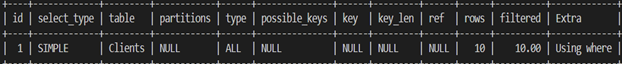
\includegraphics[width=0.8\textwidth]{./Picts/Pasted image 20251007090359.png}
    \caption{}
\end{figure}

\subsection{Penjelasan Kolom dalam Hasil EXPLAIN}
\begin{itemize}
    \item ID:

          Ini adalah pengidentifikasi urut untuk setiap pernyataan SELECT dalam kueri. Nilai ini lebih berarti ketika ada kueri bersarang (\verb|subqueries|). Dalam contoh Lucky Shrub, nilai ini adalah 1 karena ini adalah kueri sederhana.

    \item \verb|SELECT_TYPE|:

          Menampilkan jenis kueri SELECT yang akan dieksekusi. Beberapa nilai yang mungkin termasuk:
          \begin{itemize}
              \item SIMPLE: Kueri SELECT sederhana tanpa subquery atau UNION.
              \item PRIMARY: Kueri SELECT berada di luar kueri JOIN.
              \item DERIVED: Kueri SELECT adalah bagian dari subquery dalam klausa FROM.
              \item SUBQUERY: Kueri SELECT pertama dalam subquery.
              \item DEPENDENT SUBQUERY: Kueri SELECT yang bergantung pada kueri luar.
              \item UNION: Kueri SELECT adalah pernyataan kedua atau lebih dari UNION.
              \item DEPENDENT UNION: Kueri UNION yang bergantung pada kueri luar.
              \item UNION RESULT: Kueri SELECT adalah hasil dari UNION.
          \end{itemize}

    \item Table:

          Menampilkan nama tabel yang dirujuk dalam kueri SELECT. Dalam contoh Lucky Shrub, ini adalah tabel Clients.

    \item Partitions:

          Menampilkan partisi tempat data berada. Partisi memungkinkan distribusi sebagian data tabel di seluruh sistem file. Jika kueri hanya mengakses sebagian kecil data tabel, maka lebih sedikit catatan yang perlu dipindai, sehingga kueri dapat dieksekusi lebih cepat. Namun, ini lebih berarti saat berurusan dengan set data besar. Dalam contoh ini, tabel Clients tidak dipartisi, sehingga menunjukkan nilai NULL.

    \item type:
          Menunjukkan cara pencarian dilakukan. Beberapa nilai yang mungkin termasuk:
          \begin{itemize}
              \item system: Tabel hanya memiliki satu baris atau tidak ada baris.
              \item const: Nilai kolom yang dicari dapat dianggap sebagai konstanta (hanya ada satu baris yang cocok).
              \item \verb|eq_ref|: Indeks terkluster digunakan oleh operasi (indeks adalah \verb|PRIMARY KEY| atau \verb|UNIQUE INDEX|).
              \item ref: Kolom yang diindeks diakses menggunakan operator kesetaraan.
              \item fulltext: Pemindaian menggunakan indeks FULLTEXT tabel.
              \item index: Seluruh indeks dipindai untuk menemukan kecocokan.
              \item all: Seluruh tabel dipindai untuk menemukan baris yang cocok. Ini adalah jenis pemindaian terburuk dan biasanya menunjukkan kurangnya indeks yang sesuai.
          \end{itemize}

    \item \verb|possible_keys|:

          Menunjukkan kunci yang dapat digunakan oleh MySQL untuk menemukan baris dari tabel. Jika nilai kolom ini NULL, maka tidak ada indeks relevan yang ditemukan.

    \item key:

          Menunjukkan indeks yang sebenarnya digunakan oleh MySQL. Jika nilai kolom ini NULL, berarti tidak ada indeks dalam tabel yang dapat digunakan oleh optimizer.

    \item \verb|key_len|:

          Menunjukkan panjang indeks yang dipilih oleh Query Optimizer. Misalnya, nilai \verb|key_len| 4 berarti memerlukan memori untuk menyimpan empat karakter. Jika NULL, berarti tidak ada indeks yang digunakan.

    \item ref:

          Menunjukkan kolom tabel mana yang dibandingkan dengan indeks untuk melakukan pencarian. Nilai const berarti konstanta, sementara func berarti nilai yang digunakan berasal dari fungsi. Jika NULL, tidak ada kolom atau konstanta yang dibandingkan dengan indeks.

    \item rows:

          Menampilkan jumlah catatan yang diperiksa untuk menghasilkan output. Dalam contoh Lucky Shrub, hasil menunjukkan bahwa 10 catatan diperiksa, yang berarti setiap baris dalam
          tabel diperiksa. Ini menunjukkan penggunaan sumber daya database yang tidak efisien.

    \item filtered:

          Menunjukkan persentase perkiraan dari jumlah baris tabel yang telah difilter oleh kondisi tertentu. Semakin tinggi persentasenya, semakin baik kinerja kueri.

    \item Extra:

          Berisi informasi tambahan mengenai rencana eksekusi kueri. Perhatikan jika ada nilai seperti "Using temporary" atau "Using filesort" karena ini menunjukkan kueri yang bermasalah. Contoh nilai yang mungkin:
          \begin{itemize}
              \item Using temporary: Menunjukkan bahwa MySQL perlu membuat tabel sementara untuk menyimpan hasil kueri.
              \item Using filesort: Menunjukkan bahwa MySQL harus melakukan pass tambahan untuk menentukan cara mengambil baris dalam urutan yang terurut.
          \end{itemize}
\end{itemize}

\subsection{Rencana Kueri SELECT yang Lebih Efisien}
Menggunakan indeks pada kolom yang diperlukan menghasilkan kueri SELECT yang lebih efisien.

Contoh untuk menambahkan indeks pada kolom FullName:
\begin{lstlisting}[language=SQL, caption={}, captionpos=b]
CREATE INDEX IdxFullName ON Clients(FullName);
\end{lstlisting}

Sehingga hasil dari EXPLAIN akan berubah,
\begin{figure}[H]
    \centering
    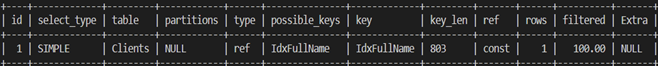
\includegraphics[width=0.8\textwidth]{./Picts/Pasted image 20251007093322.png}
    \caption{}
\end{figure}

\subsection{Pengertian Index}
\begin{itemize}
    \item Index adalah struktur data yang membantu mempertahankan pointer yang mengarah ke data yang terurut. Meskipun tidak terlihat dalam database, index dapat dibayangkan sebagai tabel dengan dua kolom: satu untuk pointer dan satu untuk data yang terurut.
    \item Indeks dibuat pada kolom tabel. Tidak semua kolom perlu diindeks; pilih kolom yang sering digunakan untuk memfilter query SELECT. Data kolom yang diindeks disimpan di lokasi terpisah yang disebut indeks, dan data diurutkan berdasarkan tipe (misalnya numerik, alfabetis, atau tanggal).
\end{itemize}

\subsection{Jenis-jenis Index}
\begin{itemize}
    \item Primary Index: Juga dikenal sebagai clustered index, disimpan dalam tabel itu sendiri dan dihasilkan secara otomatis saat tabel dibuat dengan primary atau unique key.
    \item Secondary Index: Diciptakan menggunakan pernyataan CREATE INDEX. Sintaksnya adalah:
          \begin{lstlisting}[language=SQL, caption={}, captionpos=b]
CREATE INDEX idx_column_name ON table_name (column_name);
\end{lstlisting}
    \item Index ini dapat dibuat menggunakan satu atau lebih kolom dari tabel.
\end{itemize}

\subsection{Operasi Query dan Indeks di MySQL}
\begin{itemize}
    \item Filtering rows menggunakan klausa WHERE:

          Indeks digunakan untuk mempercepat pencarian baris yang memenuhi kondisi tertentu. Jika ada beberapa indeks pada kolom yang sama, MySQL akan memilih indeks yang dapat memproses jumlah baris minimum, sehingga mengurangi waktu eksekusi.

    \item Performing JOIN operations:

          Indeks dapat digunakan untuk meningkatkan kinerja saat melakukan operasi JOIN. Untuk mendapatkan kinerja terbaik dari indeks, kolom yang digunakan dalam JOIN harus memiliki tipe data yang sama. Ini membantu MySQL dalam mengoptimalkan pencarian data yang relevan dari tabel yang berbeda.

    \item MIN dan MAX functions:

          Indeks juga dapat digunakan dengan fungsi MIN dan MAX untuk menemukan nilai minimum dan maksimum dari kolom tertentu. Ini memungkinkan query untuk lebih cepat dalam mendapatkan hasil yang diinginkan tanpa memindai seluruh tabel.

    \item Sorting and grouping operations:

          Indeks dapat digunakan dalam operasi pengurutan (ORDER BY) dan pengelompokan (GROUP BY). Dengan adanya indeks, MySQL dapat mengakses data yang sudah terurut, sehingga mempercepat proses pengurutan dan pengelompokan.
\end{itemize}

\subsection{Proses Penggunaaan Index}
\begin{itemize}
    \item Contoh Kasus: Lucky Shrub perlu mengambil nomor kontak klien dari database yang memiliki ribuan entri. Dengan menggunakan secondary index pada kolom nama lengkap, proses pencarian dapat dilakukan lebih cepat.
    \item Langkah-Langkah:
          \begin{enumerate}
              \item Gunakan pernyataan EXPLAIN untuk melihat bagaimana database mengeksekusi query.
              \item Lakukan query SELECT untuk mengambil nomor kontak yang sesuai.
              \item Jika tidak ada index, MySQL harus memindai semua baris untuk menemukan nilai yang cocok.
              \item Buat secondary index dengan sintaks:
                    \begin{lstlisting}[language=SQL, caption={}, captionpos=b]  
                CREATE INDEX idx_full_name ON clients (full_name);
            \end{lstlisting}
              \item Uji efisiensi index dengan pernyataan EXPLAIN lagi untuk melihat pengurangan jumlah baris yang dipindai.
          \end{enumerate}
\end{itemize}

\subsection{Definisi Transaksi}
Transaction adalah sekumpulan satu atau lebih query yang dapat disimpan secara permanen ke dalam database. Jika ada kesalahan, database dapat dikembalikan/rollback ke keadaan semula.

\subsection{Pernyataan Transaksi dalam MySQL}
\begin{itemize}
    \item  START TRANSACTION: Memulai proses transaksi. Ini menandai titik yang akan dikembalikan jika Anda memutuskan untuk melakukan rollback.
          \begin{lstlisting}[language=SQL, caption={}, captionpos=b]
START TRANSACTION;
\end{lstlisting}
    \item COMMIT: Menyimpan perubahan yang telah dilakukan selama transaksi ke dalam database secara permanen.
          \begin{lstlisting}[language=SQL, caption={}, captionpos=b]
COMMIT;
\end{lstlisting}
    \item ROLLBACK: Mengembalikan database ke keadaan semula jika terjadi kesalahan selama transaksi. Harus dilakukan sebelum COMMIT.
          \begin{lstlisting}[language=SQL, caption={}, captionpos=b]
ROLLBACK;
\end{lstlisting}
\end{itemize}

\subsection{Proses Pengelolaan Transaksi}
\begin{itemize}
    \item Memulai Transaksi: Gunakan START TRANSACTION untuk memulai.
    \item Menulis Query: Tambahkan query SQL yang diperlukan, seperti INSERT dan UPDATE.
    \item Menggunakan ROLLBACK: Jika terjadi kesalahan, gunakan ROLLBACK untuk mengembalikan perubahan.
    \item Menyimpan Perubahan: Jika semua query berhasil, gunakan COMMIT untuk menyimpan perubahan.
\end{itemize}

\subsection{Contoh Kasus Transaksi}
Lucky Shrub melakukan pembaruan pada tabel pesanan dan produk. Jika terjadi kesalahan, mereka dapat menggunakan ROLLBACK untuk mengembalikan data ke keadaan semula.

\subsection{Definisi CTE(Common Table Expression)}
CTE adalah metode untuk mengoptimalkan kueri database yang kompleks dengan mengompilasi mereka menjadi blok kode sederhana yang dapat digunakan kembali. Bisa dipahami sebagai cara untuk membuat tabel sementara yang akan segera dihapus setelah query selesai.

CTE tidak menyimpan data secara permanen di database; sebaliknya, ia berfungsi sebagai "tabel virtual" yang hanya ada untuk durasi kueri yang sedang dijalankan. Setelah kueri selesai dieksekusi, data dalam CTE tidak lagi tersedia, mirip dengan tabel sementara yang dihapus setelah sesi berakhir.

\subsection{Penggunaan CTE}
\begin{itemize}
    \item CTE membantu menyederhanakan kueri yang rumit, membuatnya lebih mudah dibaca dan dikelola.
    \item CTE dapat dibuat untuk satu atau beberapa kueri, tergantung pada kebutuhan database.
\end{itemize}

\subsection{Sintaks untuk CTE Tunggal}
\begin{lstlisting}[language=SQL, caption={}, captionpos=b]
WITH cte_name AS (
    -- query
)
SELECT * FROM cte_name;
\end{lstlisting}
\begin{itemize}
    \item \verb|cte_name|: Nama yang diberikan untuk CTE.
    \item AS: Kata kunci yang mengaitkan kueri dengan nama CTE.
\end{itemize}

\subsection{Sintaks untuk CTE Ganda}
\begin{lstlisting}[language=SQL, caption={}, captionpos=b]
WITH cte_name1 AS (
    -- query1
), cte_name2 AS (
    -- query2
)
SELECT * FROM cte_name1
UNION
SELECT * FROM cte_name2;
\end{lstlisting}
\begin{itemize}
    \item Setiap kueri harus memiliki nama unik dan dipisahkan dengan koma.
    \item Gunakan UNION untuk menggabungkan hasil dari beberapa CTE.
\end{itemize}

\subsection{Pengertian Prepared Statement}
Prepared Statement adalah sebuah pernyataan SQL yang telah dikompilasi dan dapat digunakan berulang kali tanpa perlu dikompilasi ulang setiap kali. Ini menghemat sumber daya MySQL.

\subsection{Proses Membuat dan Menjalankan Prepared Statement}
\begin{enumerate}
    \item Langkah 1: Siapkan pernyataan menggunakan perintah \verb|PREPARE|.
          \begin{lstlisting}[language=SQL, caption={}, captionpos=b]
    PREPARE statement_name FROM 'SELECT * FROM orders WHERE order_id = ?';
    \end{lstlisting}
    \item Langkah 2: Tentukan variabel untuk parameter yang tidak ditentukan. \verb|@order_id|: Variabel yang menyimpan nilai untuk parameter dalam prepared statement.
          \begin{lstlisting}[language=SQL, caption={}, captionpos=b]
    SET @order_id = 10;
    \end{lstlisting}
    \item Langkah 3: Eksekusi pernyataan menggunakan perintah \verb|EXECUTE|. Ini akan menjalankan prepared statement dengan nilai yang ditentukan.
          \begin{lstlisting}[language=SQL, caption={}, captionpos=b]
    EXECUTE statement_name USING @order_id;
    \end{lstlisting}
\end{enumerate}

\subsection{Keuntungan Menggunakan Prepared Statement}
\begin{itemize}
    \item Efisiensi: Mengurangi beban pada server MySQL karena pernyataan hanya dikompilasi sekali.
    \item Keamanan: Mengurangi risiko serangan SQL injection karena parameter tidak langsung disisipkan ke dalam pernyataan SQL.
\end{itemize}

\subsection{JSON dalam MySQL}
\begin{itemize}
    \item JSON (JavaScript Object Notation): Format teks yang digunakan untuk menyimpan dan mentransfer data. JSON mudah dibaca dan tidak memerlukan pemrosesan khusus.
    \item Contoh Sintaks: Dalam pernyataan INSERT INTO, JSON ditulis dalam tanda kutip tunggal dan kurung kurawal. Setiap properti dan nilai ditulis dalam tanda kutip ganda dan dipisahkan oleh titik dua, dengan setiap pasangan dipisahkan oleh koma.
          \begin{lstlisting}[language=SQL, caption={}, captionpos=b]
INSERT INTO activity (activity_id, properties) VALUES
(1, '{"clientID": "123", "productID": "456", "order": true}'),
(2, '{"clientID": "124", "productID": "457", "order": false}'),
(3, '{"clientID": "125", "productID": "458", "order": true}');
\end{lstlisting}
\end{itemize}

\subsection{Penggunaan JSON dalam MySQL}
\begin{enumerate}
    \item Membuat Tabel

          Untuk membuat tabel yang menyimpan aktivitas klien, Anda dapat menggunakan sintaks berikut:
          \begin{lstlisting}[language=SQL, caption={}, captionpos=b]
CREATE TABLE activity (
    activity_id INT PRIMARY KEY,
    properties JSON
);
\end{lstlisting}
    \item Menyisipkan Data

          Untuk menyisipkan data ke dalam tabel menggunakan JSON, sintaksnya adalah:
          \begin{lstlisting}[language=SQL, caption={}, captionpos=b]
INSERT INTO activity (activity_id, properties) VALUES
(1, '{"clientID": "123", "productID": "456", "order": true}'),
(2, '{"clientID": "124", "productID": "457", "order": false}'),
(3, '{"clientID": "125", "productID": "458", "order": true}');
\end{lstlisting}

    \item Mengambil Data

          Untuk mengambil data dari kolom properties, Anda dapat menggunakan sintaks berikut:
          \begin{lstlisting}[language=SQL, caption={}, captionpos=b]
SELECT activity_id, properties 
FROM activity 
WHERE properties->'$.clientID' = '123';
\end{lstlisting}
\end{enumerate}

Penjelasan Sintaks:
\begin{itemize}
    \item CREATE TABLE: Digunakan untuk membuat tabel baru dalam database.
    \item INSERT INTO: Digunakan untuk menyisipkan data baru ke dalam tabel.
    \item SELECT: Digunakan untuk mengambil data dari tabel.
    \item \verb|properties->'$.clientID'|: Menggunakan operator jalur kolom untuk mengakses elemen dalam data JSON.
\end{itemize}

Nilai JSON selalu diapit dengan dua tanda petik. Untuk mendapatkan nilai sebuah key tanpa tanda petik bisa gunakan \verb|properties->>'$.value'|. Sebaliknya, \verb|properties->'$.value'| akan mengembalikan nilai JSON dengan tanda petik

\subsection{Penjelasan Lebih Lanjut terkait Teknik Optimasi MySQL}
\subsubsection{Ringkasan}
Seperti yang mungkin sudah Anda ketahui, teknik optimasi database digunakan untuk meningkatkan kinerja database Anda. Pada pelajaran sebelumnya, Anda telah belajar cara mengoptimalkan kueri SELECT MySQL menggunakan berbagai teknik yang berbeda.

Namun, ada teknik optimasi lain yang dapat digunakan untuk mendukung optimasi database Anda, seperti transaksi, ekspresi tabel umum, dan pernyataan yang disiapkan.

Anda mungkin sudah menemui teknik-teknik ini dalam pelajaran ini. Jadi, mari kita luangkan waktu sejenak untuk memahami dasar-dasar bagaimana teknik-teknik ini digunakan untuk mengoptimalkan kueri database.

\subsubsection{MySQL Transaction}
Sebagai seorang insinyur basis data, Anda harus menggunakan transaksi MySQL setiap kali Anda memiliki aktivitas kritis yang perlu diselesaikan. Jika terjadi kesalahan selama eksekusi kueri, Anda dapat menggunakan teknik ini untuk mengembalikan basis data ke keadaan semula.

Teknik ini sangat berguna untuk dipertimbangkan saat menulis serangkaian kueri terkait yang harus dieksekusi sesuai rencana untuk mencapai hasil yang diharapkan.

Misalnya, Lucky Shrub telah menulis serangkaian kueri untuk membantu dalam pemrosesan pesanan baru. Saat pesanan diterima, database terlebih dahulu memeriksa apakah ada cukup barang tersedia di stok untuk memenuhi pesanan. Setelah pesanan diproses, database kemudian memperbarui jumlah barang yang tersisa di stok.

Ada banyak langkah dalam proses ini. Dan beberapa perubahan, atau operasi yang diperlukan, mungkin gagal terjadi di database. Jika demikian, Lucky Shrub dapat menggunakan transaksi MySQL untuk membatalkan perubahan dan membatalkan transaksi saat ini jika ada pernyataan yang gagal dieksekusi sesuai yang diperlukan.

Anda dapat menggunakan alias MySQL BEGIN atau BEGIN WORK untuk memulai transaksi MySQL. Meskipun perintah START TRANSACTION adalah cara standar untuk memulai proses transaksi di MySQL.

Kemudian ketikkan pernyataan SELECT yang diperlukan. Jika semua kueri dieksekusi sesuai harapan, maka pernyataan COMMIT digunakan untuk mengonfirmasi transaksi saat ini dan membuat perubahan transaksi menjadi permanen.

Namun, salah satu atau lebih dari pernyataan ini mungkin gagal dieksekusi sesuai yang diharapkan. Jika demikian, Anda dapat menggunakan pernyataan ROLLBACK untuk membatalkan transaksi saat ini, membatalkan perubahan yang dilakukan pada database, dan mengembalikannya ke keadaan semula.

Proses ini dijelaskan dalam sintaks abstrak berikut:
\begin{lstlisting}[language=SQL, caption={}, captionpos=b]
START TRANSACTION; 
SQL statements 
ROLLBACK; 
\end{lstlisting}

\subsubsection{Common Table Expressions}
Insinyur basis data sering kali perlu menulis kueri SQL yang kompleks, yang biasanya sulit dibaca dan dipelihara.

Dalam situasi ini, Anda dapat menggunakan teknik Common Table Expression (CTE) untuk memecah kueri kompleks menjadi blok-blok kode yang sederhana. Dengan CTE, Anda dapat menulis ulang kueri tersebut dengan cara yang menyederhanakannya dan membuatnya lebih mudah dibaca dan dipelihara.

Sintaks abstrak dasar dari Common Table Expression adalah sebagai berikut:
\begin{lstlisting}[language=SQL, caption={}, captionpos=b]
WITH CTE_Name AS (query code)  
SELECT * 
FROM CTE_Name; 
\end{lstlisting}

Dalam sintaks ini, Anda menggunakan klausa WITH untuk memulai ekspresi tabel umum, diikuti dengan nama ekspresi tabel umum tersebut. Nama ini dapat disesuaikan.

Selanjutnya, gunakan kata kunci AS untuk mengaitkan kueri dengan nama ekspresi terkait. Terakhir, gunakan pernyataan SELECT untuk mengakses nama ekspresi tabel umum.

Jika Anda memerlukan beberapa kueri, Anda hanya perlu mengaitkan setiap kueri dengan nama ekspresi terkaitnya dan memisahkannya dengan koma, seperti pada contoh berikut:

\begin{lstlisting}[language=SQL, caption={}, captionpos=b]
WITH 
  cte1 AS (query1), 
  cte2 AS (query2) 
SELECT cte1  UNION cte2;
\end{lstlisting}

Sintaks abstrak ini menentukan dua ekspresi tabel umum yang dipisahkan oleh koma. Setiap ekspresi terkait dengan kueri menggunakan kata kunci AS.

\subsubsection{Prepared statements}
Sebuah kueri harus diparsing oleh MySQL sebelum dapat dieksekusi, yang memakan waktu dan menyebabkan penundaan.

Namun, pembuatan pernyataan siap pakai (prepared statements) di MySQL dapat mengurangi waktu parsing kueri. Pernyataan siap pakai hanya perlu diparsing oleh MySQL sekali, terlepas dari berapa kali pernyataan tersebut digunakan dan dieksekusi.

Pernyataan yang disiapkan di MySQL adalah templat yang Anda buat dengan pernyataan SQL. Pernyataan yang disiapkan dimulai dengan perintah PREPARE diikuti oleh nama pernyataan. Nama ini dapat disesuaikan. Pernyataan ini juga dapat mencakup nilai-nilai yang tidak ditentukan, yang digunakan sebagai parameter dan dilabeli dengan tanda tanya \verb|?|

Misalnya, dalam sintaks berikut, dua tanda tanya \verb|?| mewakili dua parameter yang dapat digunakan untuk menyisipkan dua nilai berbeda ke dalam tabel Products:
\begin{lstlisting}[language=SQL, caption={}, captionpos=b]
PREPARE InsertProductData FROM 'INSERT INTO Products VALUES(?, ?)'; 
\end{lstlisting}

Pernyataan yang telah disiapkan juga meminimalkan penggunaan bandwidth saat mengomunikasikan data dengan server MySQL. Anda hanya perlu meneruskan nilai parameter ke pernyataan yang telah disiapkan, bukan seluruh pernyataan SQL.

Membuat pernyataan yang telah disiapkan juga mengamankan basis data Anda dari injeksi SQL, teknik peretasan umum yang dapat digunakan untuk menghancurkan basis data Anda. Injeksi SQL mencoba mengirimkan kode berbahaya ke basis data Anda melalui pernyataan SQL. Namun, hal ini dapat dihindari jika Anda menggunakan pernyataan yang telah disiapkan saat membuat kueri SQL.

\section{MySQL for data analytics}
\subsection{Data Analysis vs. Data Analytics}
Data Analysis adalah proses mengumpulkan dan memeriksa data untuk mendapatkan wawasan. Sedangkan Data Analytics adalah mengambil langkah lebih lanjut dengan mengolah data yang telah dianalisis menjadi informasi yang berguna untuk pengambilan keputusan bisnis.

Data Analysis dan Data Analytics adalah konsep yang saling terkait; Anda tidak dapat melakukan data analytics tanpa melakukan data analysis terlebih dahulu.

\subsection{Jenis-jenis Data Analysis}
\begin{itemize}
    \item Descriptive Data Analysis

          Menyajikan data dalam format deskriptif. Contoh: Menganalisis penjualan Lucky Shrub selama periode tertentu untuk menjelaskan produk terlaris dan keuntungan.
    \item Exploratory Data Analysis

          Mencoba menemukan hubungan antara variabel yang berbeda. Contoh: Menentukan apakah ada korelasi antara peningkatan penjualan produk tertentu dan musim penjualannya.
    \item Inferential Data Analysis

          Menggunakan sampel kecil data untuk menarik kesimpulan tentang populasi yang lebih besar. Contoh: Menggunakan data penjualan untuk menyimpulkan bahwa musim panas adalah waktu terbaik untuk menjual produk barbecue.
    \item Predictive Data Analysis

          Menggunakan data yang ada untuk mengidentifikasi pola dan membuat prediksi tentang kinerja di masa depan. Contoh: Memprediksi bahwa diskon pada alat berkebun akan meningkatkan penjualan.
    \item Causal Data Analysis

          Meneliti hubungan sebab-akibat antara variabel. Contoh: Menganalisis apakah pembelian alat berkebun mempengaruhi pembelian produk pencahayaan luar ruangan.
\end{itemize}

\subsection{Perihal Data Analytics}
Analisis data merupakan isu penting bagi berbagai jenis organisasi di berbagai sektor, termasuk pendidikan, pemerintahan, kesehatan, pariwisata, dan bisnis.

Analisis data berfokus pada pengumpulan, pengolahan, dan penyelidikan data untuk memperoleh wawasan mendalam tentang kinerja suatu organisasi. Misalnya, sebuah bisnis dapat menggunakan analisis data untuk memahami pola penjualan, perilaku pelanggan, atau margin keuntungan mereka.

Analisis data menyediakan informasi yang berguna dan bermakna yang dapat dimanfaatkan oleh pengambil keputusan dalam organisasi untuk mengatasi masalah dan tantangan pada tahap awal. Hal ini juga membantu mereka memprediksi masa depan organisasi mereka.

\subsection{Manfaat MySQL}
Database MySQL dibangun menggunakan model relasional. Model ini menyimpan kumpulan data dalam tabel-tabel yang saling terkait, sehingga memudahkan akses, pemrosesan, dan analisis data yang ada.

Ini juga merupakan sistem manajemen basis data sumber terbuka yang dapat menyimpan jumlah data yang sangat besar. Dalam analisis basis data, semakin banyak data yang disimpan dan diproses oleh basis data Anda, semakin baik hasil analisis Anda.

MySQL digunakan secara luas oleh berbagai jenis bisnis, platform media sosial, aplikasi e-commerce, dan situs web pemerintah. Hal ini berarti organisasi-organisasi tersebut dapat dengan mudah mengintegrasikan data yang diimpor dari berbagai sumber, yang akan memfasilitasi lingkungan data yang kaya untuk melakukan analisis data.

\begin{itemize}
    \item Relational Database Model: MySQL menggunakan model basis data relasional, yang menyusun data dalam tabel terkait, memudahkan akses dan analisis informasi.
    \item Foreign Keys: MySQL memungkinkan penghubungan tabel menggunakan foreign keys, seperti menghubungkan tabel pesanan dan produk melalui product ID key.
\end{itemize}

\subsection{Keterbatasan MySQL}
\begin{itemize}
    \item Keterbatasan Analisis Data: MySQL memiliki kemampuan analisis data yang lebih terbatas dibandingkan dengan alat analisis data yang lebih canggih.
    \item Kurangnya Fitur Visualisasi: MySQL tidak memiliki fitur visualisasi data seperti grafik atau peta, yang dapat membantu dalam mengidentifikasi tren dan masalah.
\end{itemize}

\subsection{MySQL dan alat analitik data canggih}
Kemampuan MySQL dalam melakukan analisis data cukup memadai. Namun, kapasitasnya untuk pemrosesan analisis canggih jauh lebih terbatas dibandingkan dengan alat analisis canggih lainnya.

MySQL lebih berfokus pada pemrosesan transaksi data daripada analisis, di mana catatan data dikelola dalam tabel melalui baris dan kolom menggunakan operasi SQL seperti INSERT, UPDATE, dan DELETE.

Pemilik bisnis dan manajer perlu melakukan operasi analitik data yang canggih. Oleh karena itu, mereka sering mengintegrasikan MySQL dengan platform analitik canggih lainnya untuk memaksimalkan manfaat analitik data.

Platform-platform lain ini menyediakan antarmuka pengguna yang ramah untuk menangani data. Mereka juga menampilkan data yang dianalisis dalam berbagai format visual seperti grafik, diagram, peta, dan dasbor interaktif.

Menghasilkan data atau informasi dalam format visual ini merupakan metode yang berguna untuk mengidentifikasi tren, celah, pola, dan model. Hal ini jauh lebih mudah daripada bekerja dengan data mentah dalam tabel, karena informasi visual dapat diproses oleh otak manusia dengan jauh lebih cepat.

MySQL dapat diintegrasikan dengan berbagai alat analitik canggih, termasuk dua platform paling populer, Tableau dan Power BI. Tableau adalah platform analitik paling populer di dunia. Power BI adalah alat visualisasi data interaktif penting yang dikembangkan oleh Microsoft. Fokus utamanya adalah pada intelijen bisnis.

Baik Tableau maupun Power BI adalah alat visualisasi canggih yang digunakan untuk mengakses, menghubungkan, dan menganalisis data dari berbagai sumber. Mereka kemudian dapat mengubah data yang dianalisis menjadi dasbor interaktif.

Platform-platform ini juga dilengkapi dengan konektor bawaan yang memudahkan integrasi, visualisasi, dan analisis data MySQL dengan mendukung mekanisme Select, Extract, Transform, dan Load (SETL).

Alat-alat ini dapat digunakan untuk dengan mudah mengidentifikasi data MySQL yang akan dianalisis. Mereka mengekstrak data yang dipilih, mengubahnya menjadi format yang sesuai, dan memuat data tersebut ke platform untuk melakukan berbagai jenis analisis data.

\subsection{Pengantar Analisis Data}
Analisis Data adalah proses mengumpulkan dan mempresentasikan data untuk mendapatkan wawasan. SQL Queries adalah kumpulan perintah yang digunakan untuk mengakses dan memanipulasi data dalam database.

\subsection{Proses Analisis Data}
\begin{itemize}
    \item Ekstraksi Data: Mengambil data yang diperlukan dari database menggunakan SQL queries.
    \item Deskripsi Hasil: Menggunakan SQL queries tambahan untuk menjelaskan hasil analisis data.
    \item Wawasan Lebih Lanjut: Menggunakan data yang diekstrak untuk mendapatkan wawasan lebih dalam melalui analisis data.
\end{itemize}

\subsection{Pengantar FULL OUTER JOIN}
FULL OUTER JOIN adalah proses mengembalikan semua catatan dari tabel kiri dan tabel kanan, termasuk catatan yang cocok dan yang tidak cocok. MySQL tidak mendukung FULL OUTER JOIN, sehingga cara kerjanya perlu ditiru menggunakan kombinasi LEFT JOIN dan RIGHT JOIN.

\subsection{Sintaks untuk Meniru FULL OUTER JOIN}
\begin{itemize}
    \item Menggunakan UNION ALL:
          \begin{lstlisting}[language=SQL, caption={}, captionpos=b]
SELECT column1, column2 FROM table1
LEFT JOIN table2 ON table1.id = table2.id
UNION ALL
SELECT column1, column2 FROM table1
RIGHT JOIN table2 ON table1.id = table2.id;
\end{lstlisting}

          UNION ALL: Menggabungkan hasil dari dua query dan mengembalikan semua catatan, termasuk duplikat.
    \item Menggunakan UNION:
          \begin{lstlisting}[language=SQL, caption={}, captionpos=b]
SELECT column1, column2 FROM table1
LEFT JOIN table2 ON table1.id = table2.id
UNION
SELECT column1, column2 FROM table1
RIGHT JOIN table2 ON table1.id = table2.id;
\end{lstlisting}

          UNION: Menggabungkan hasil dari dua query dan mengembalikan hanya catatan unik.
\end{itemize}

\subsection{Query JOIN dengan 3 Tabel}
\subsubsection{Contoh Kasus: Lucky Shrub}
\begin{itemize}
    \item Tujuan: Mengidentifikasi semua klien yang membeli 10 item atau lebih dari lini produk tertentu untuk mengirimkan penawaran khusus.
    \item Kriteria:
          \begin{itemize}
              \item Pembelian harus dilakukan setelah 5 September 2020.
              \item Tersedia 50 unit atau lebih dari produk di stok.
          \end{itemize}
\end{itemize}

\subsubsection{Tabel yang Terlibat}
\begin{enumerate}
    \item Orders Table: Menyimpan informasi tentang setiap pesanan.
    \item Clients Table: Menyimpan informasi penting tentang setiap klien.
    \item Products Table: Menyimpan data tentang semua produk di toko.
\end{enumerate}

\subsubsection{Langkah-langkah Query}
\begin{itemize}
    \item SELECT Statement: Mulai dengan pernyataan SELECT untuk memilih kolom yang diperlukan.
          \begin{lstlisting}[language=SQL, caption={}, captionpos=b]
    SELECT clients.client_id, clients.contact_number, orders.order_id, orders.quantity, orders.date, products.number_of_items AS items_in_stock
    \end{lstlisting}
    \item FROM dan INNER JOIN: Gunakan kata kunci FROM untuk menargetkan tabel klien dan INNER JOIN untuk menggabungkan dengan tabel orders dan products.
          \begin{lstlisting}[language=SQL, caption={}, captionpos=b]
    FROM clients INNER JOIN orders ON clients.client_id = orders.client_id INNER JOIN products ON orders product_id = products.product_id
    \end{lstlisting}
    \item WHERE Clause: Tambahkan klausa WHERE untuk menetapkan kriteria.
          \begin{lstlisting}[language=SQL, caption={}, captionpos=b]
    WHERE orders.quantity >= 10 AND orders.date > '2020-09-05' AND products.number_of_items >= 50
    \end{lstlisting}
    \item Eksekusi Query: Klik Enter untuk menjalankan query dan menampilkan data yang diperlukan.
\end{itemize}

\end{document}